% !TeX encoding = UTF-8 Unicode 
%Tiedoston merkistö

\documentclass[finnish]{article}


\usepackage{pgf}
\usepackage{tikz}
\usetikzlibrary{arrows,automata}

\usepackage{babel,t1enc} %,times} % Suomen tavutus

\usepackage[utf8]{inputenc} % näppäimiltä tuleva merkistö
\usepackage{geometry}
\geometry{margin=2cm,a4paper}  % paperin koko
%\geometry{margin=2.54cm}

\usepackage{lastpage}
\usepackage{fancyhdr}
\pagestyle{fancy}
\fancyhf{} % clear all header and footer fields
\renewcommand{\headrulewidth}{0pt}
\cfoot{\thepage\ (\pageref{LastPage})}


\usepackage{amssymb,amsmath,mycode}
%\input{../macs/macs}
%\input{bwmacs}


\usepackage{graphicx}

\newcommand{\set}[1]{{\left\{ #1 \right\}}}


\begin{document}

\subsection*{582206 Laskennan mallit (syksy 2012)\\
{\rm Harjoitus 2 (10.--13.9.)}}


\begin{enumerate}


\item Olkoon kahden äärellisen automaatin $M_1$ ja $M_2$ tilat ja siirtymät seuraavat. 

\begin{tabular}{cc}
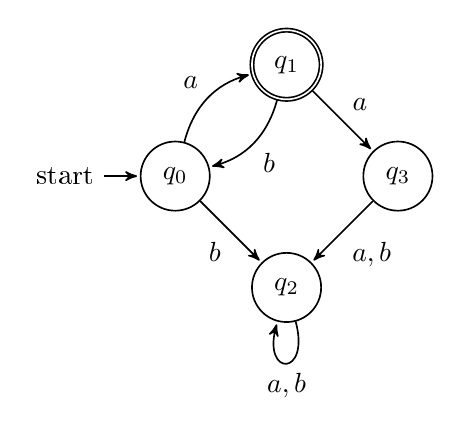
\begin{tikzpicture}[->,>=stealth',shorten >=1pt,auto,node distance=2cm,semithick]
 %\tikzstyle{every state}=[fill=red,draw=none,text=white]

 \node[initial,state]  (q0)                     {$q_0$};
 \node[state,accepting](q1) [above right of=q0] {$q_1$};
 \node[state]          (q2) [below right of=q0] {$q_2$};
 \node[state]          (q3) [above right of=q2] {$q_3$};

 \path (q0) edge [bend left]  node       {$a$} (q1)
            edge              node [swap]{$b$} (q2)
       (q1) edge              node       {$a$} (q3)
            edge [bend left] node        {$b$} (q0)
       (q2) edge [loop below] node {$a,b$} ()
       (q3) edge             node {$a,b$} (q2);
\end{tikzpicture} 
&
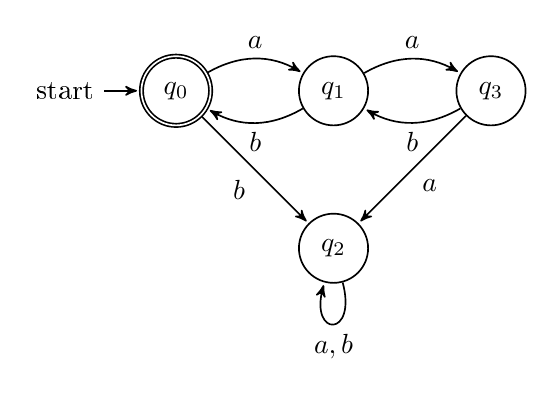
\begin{tikzpicture}[->,>=stealth',shorten >=1pt,auto,node distance=2cm,semithick]
 %\tikzstyle{every state}=[fill=red,draw=none,text=white]

 \node[initial,state,accepting]
              (q0)               {$q_0$};
 \node[state]           (q1) [right of=q0] {$q_1$};
 \node[state] (q2) [below of=q1] {$q_2$};
 \node[state] (q3) [right of=q1] {$q_3$};

 \path (q0) edge [bend left]  node       {$a$}   (q1)
            edge              node [swap]{$b$}   (q2)
       (q1) edge [bend left]  node       {$a$}  (q3)
            edge [bend left]  node       {$b$}   (q0)
       (q2) edge [loop below] node       {$a,b$} ()
       (q3) edge              node       {$a$}   (q2)
       (q3) edge [bend left]  node       {$b$} (q1);
\end{tikzpicture}
\\
$M_1$ & $M_2$
\end{tabular}
\begin{enumerate}
\item Mikä on kukin automaatin aloitustila?
\item Mitkä ovat hyväksyviä tiloja?
\item Minkä tilajonon automaatit käyvät läpi syötteellä $aabb$
\item Hyväksyvätkö automaatit syötteen $aabb$?
\item Hyväksyvätkö automaatit merkkijonon $\varepsilon$ (tyhjä merkkijono)?
\end{enumerate}

\item Olkoon äärellisen automaatin $M$ formaali kuvaus $(\set{q_1,q_2,q_3,q_4,q_5}, \set{u,d}, \delta, q_3, \set{q_3})$ missä siirtymäfunktion määrittelee taulukko:
\[
\begin{array}{c|cc}
    & u   & d   \\ \hline
q_1 & q_1 & q_2 \\
q_2 & q_1 & q_3 \\
q_3 & q_2 & q_4 \\
q_4 & q_3 & q_5 \\
q_5 & q_4 & q_5
 \end{array} 
\]
Piirrä automaatti $M$ (tilat ja siirtymät).

\item Minkälaisia merkkijonoja eli sanoja seuraavat äärelliset automaatit hyväksyvät?



\begin{tabular}{cccc}
(a) & 
\begin{tabular}{c}
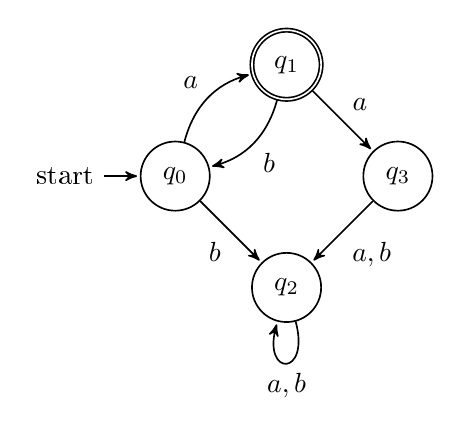
\begin{tikzpicture}[->,>=stealth',shorten >=1pt,auto,node distance=2cm,semithick]
 %\tikzstyle{every state}=[fill=red,draw=none,text=white]

 \node[initial,state]  (q0)                     {$q_0$};
 \node[state,accepting](q1) [above right of=q0] {$q_1$};
 \node[state]          (q2) [below right of=q0] {$q_2$};
 \node[state]          (q3) [above right of=q2] {$q_3$};

 \path (q0) edge [bend left]  node       {$a$} (q1)
            edge              node [swap]{$b$} (q2)
       (q1) edge              node       {$a$} (q3)
            edge [bend left] node        {$b$} (q0)
       (q2) edge [loop below] node {$a,b$} ()
       (q3) edge             node {$a,b$} (q2);
\end{tikzpicture} 
\end{tabular}
& (b) &
\begin{tabular}{c}
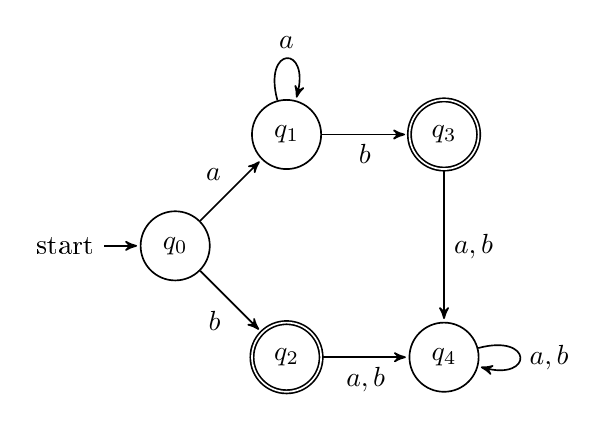
\begin{tikzpicture}[->,>=stealth',shorten >=1pt,auto,node distance=2cm,semithick]
 %\tikzstyle{every state}=[fill=red,draw=none,text=white]

 \node[initial,state]   (q0)                     {$q_0$};
 \node[state]           (q1) [above right of=q0] {$q_1$};
 \node[state,accepting] (q2) [below right of=q0] {$q_2$};
 \node[state,accepting] (q3) [right of=q1]       {$q_3$};
 \node[state]           (q4) [right of=q2]       {$q_4$};

 \path (q0) edge              node       {$a$}   (q1)
            edge              node [swap]{$b$}   (q2)
       (q1) edge [loop above] node       {$a$}   ()
            edge              node [swap]{$b$}   (q3)
       (q2) edge              node [swap]{$a,b$} (q4)
       (q3) edge              node       {$a,b$} (q4)
       (q4) edge [loop right] node       {$a,b$} ();    
\end{tikzpicture}
\end{tabular}
\end{tabular}

\begin{tabular}{cccc}
(c) &
\begin{tabular}{c}
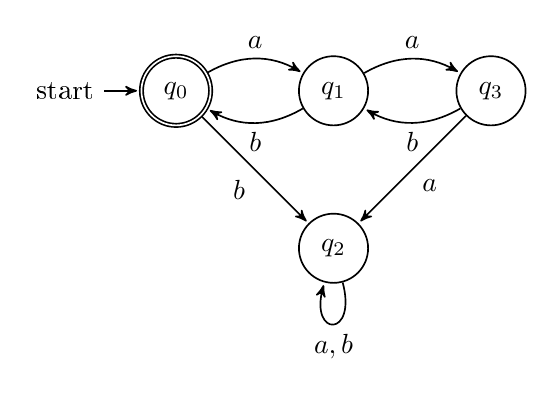
\begin{tikzpicture}[->,>=stealth',shorten >=1pt,auto,node distance=2cm,semithick]
 %\tikzstyle{every state}=[fill=red,draw=none,text=white]

 \node[initial,state,accepting]
              (q0)               {$q_0$};
 \node[state]           (q1) [right of=q0] {$q_1$};
 \node[state] (q2) [below of=q1] {$q_2$};
 \node[state] (q3) [right of=q1] {$q_3$};

 \path (q0) edge [bend left]  node       {$a$}   (q1)
            edge              node [swap]{$b$}   (q2)
       (q1) edge [bend left]  node       {$a$}  (q3)
            edge [bend left]  node       {$b$}   (q0)
       (q2) edge [loop below] node       {$a,b$} ()
       (q3) edge              node       {$a$}   (q2)
       (q3) edge [bend left]  node       {$b$} (q1);
\end{tikzpicture}
\end{tabular}
& (d) &
\begin{tabular}{c}
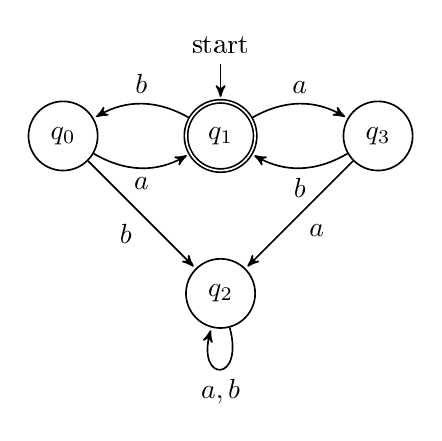
\begin{tikzpicture}[->,>=stealth',shorten >=1pt,auto,node distance=2cm,semithick]
 %\tikzstyle{every state}=[fill=red,draw=none,text=white]

 \node[state] (q0)               {$q_0$};
 \node[state,initial above,accepting]
              (q1) [right of=q0] {$q_1$};
 \node[state] (q2) [below of=q1] {$q_2$};
 \node[state] (q3) [right of=q1] {$q_3$};

 \path (q0) edge [bend right]  node [swap]{$a$}   (q1)
            edge              node [swap]{$b$}   (q2)
       (q1) edge [bend left]  node       {$a$}  (q3)
            edge [bend right]  node [swap]{$b$}   (q0)
       (q2) edge [loop below] node       {$a,b$} ()
       (q3) edge              node       {$a$}   (q2)
       (q3) edge [bend left]  node       {$b$} (q1);
\end{tikzpicture}
\end{tabular}
\end{tabular}

\begin{tabular}{cccc}
(e) &
\begin{tabular}{c}
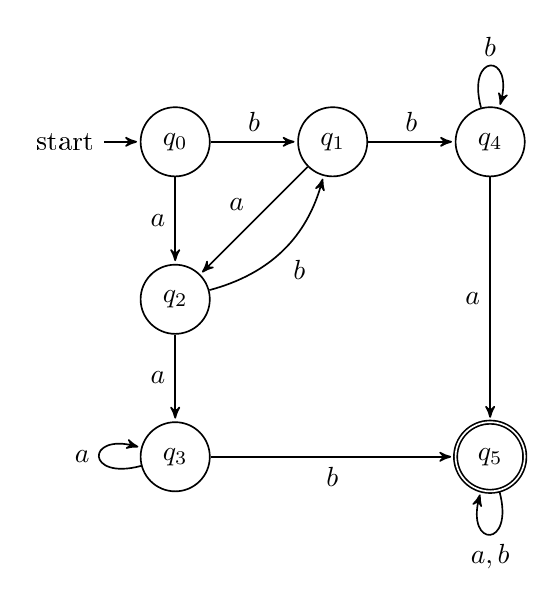
\begin{tikzpicture}[->,>=stealth',shorten >=1pt,auto,node distance=2cm,semithick]
 %\tikzstyle{every state}=[fill=red,draw=none,text=white]

 \node[state,initial] (q0)               {$q_0$};
 \node[state]       (q1) [right of=q0] {$q_1$};
 \node[state]       (q2) [below of=q0] {$q_2$};
 \node[state]       (q3) [below of=q2] {$q_3$};
 \node[state]       (q4) [right of=q1]  {$q_4$};
 \node              (qx)[below of=q4] {};
 \node[state,accepting](q5)[below of=qx] {$q_5$};
 
 \path (q0) edge              node [swap]{$a$}   (q2)
            edge              node       {$b$}   (q1)
       (q1) edge              node [swap] {$a$}  (q2)
            edge              node      {$b$}   (q4)
       (q2) edge              node [swap] {$a$} (q3)
            edge [bend right] node [swap] {$b$} (q1)
       (q3) edge [loop left]  node       {$a$}   ()
       (q3) edge              node [swap]{$b$} (q5)
       (q4) edge              node [swap]{$a$} (q5)
       (q4) edge [loop above] node      {$b$} ()
       (q5) edge [loop below] node       {$a,b$} ();
\end{tikzpicture}
\end{tabular}
\end{tabular}


\item Piirrä äärelliset automaatit tiloineen ja siirtymänuolineen seuraaville kielille.
\begin{enumerate}
\item $L = \set{w \in \set{a, b}^* \mid \mbox{$w$ sisältää ainakin yhden $a$:n}}$
\item $L = \set{w \in \set{a, b}^* \mid \mbox{$w$ alkaa $b$ tai $ab$:llä}}$
\item $L = \set{w \in \set{a,b}^*  \mid \mbox{$w$ loppuu $aa$:han}}$
\item $L = \set{w \in \set{a,b}^* \mid \mbox{ $w$ sisältää merkkijonon $abab$ }}$
\item $L = \set{w \in \set{a,b}^* \mid \mbox{ jokaisen $w$:ssä olevan $a$:n edessa on $b$}}$
%\item $L = \set{w \in \set{a,b}^* \mid \mbox{ $w$ ei sisällä merkkijonoa $aa$ eikä merkkijonoa $bb$  }}$ 
%\item $L = \set{w \in \set{a,b}^* \mid \mbox{ $w$ sisältää parittoman määrän kirjainta $a$ ja parillisen määrän kirjainta $b$ }}$
%\item $L = \set{w \in \set{a,b}^* \mid \mbox{ $w$ sisältää sekä merkkijonon $ab$ että $ba$:n}}$
\end{enumerate}

\item
Olkoon kielet $A$ ja $B$ säännöllisiä. Todista että joukkoerotus $A - B$ tuottaa säännöllisen kielen luentokalvojen yhdisteen esimerkin mukaisesti. Piirrä myös pieni esimerkki automaateista $L(M_1)=A$, $L(M_2)= B$ ja $L(M_{A-b})=A-B$ .

\item
Seuraavat kielet koostettu yksinkertaisemmista kielistä säännöllisillä operaatioilla (kaikkia ei vielä todistettu tunnilla). Piirrä jokaisessa kohdassa ensin yksinkertaiset kielet tunnistavat automaatit tiloineen ja siirtymineen ja piirrä sen perusteella lopullinen automaatti (vrt. luentokalvojen yhdisteautomaatti). Kaikissa kohdissa $\Sigma = \set{a,b}$
\begin{enumerate}
\item 
$\set{w \mid \mbox{$w$ sisältää ainakin kolme $a$:ta ja ainakin kaksi $b$:tä}}$
\item
$\set{w \mid \mbox{$w$:n pituus on parillinen sisältäen parittoman määrän $a$:ta} }$
\item 
$\set{w \mid \mbox{$w$:ssä olevin $a$-merkkien määrä ei ole kaksi} }$
\item 
$\set{w \mid \mbox{$w$ ei sisällä alimerkkijonoja $ab$ ja $ba$} }$
\item
$\set{w \mid \mbox{$w$ on mikä tahansa muu merkkijono kuin $a$ tai $b$} }$ 
\end{enumerate}



\end{enumerate}

\end{document}
